    \section{Εισαγωγή}

Σήμα - σύστημα
	\begin{align*}
	\boxed{\quad \underbrace{g}_{{\text{εξαρτημένη}}} = f(\underbrace{t}_{{\text{ανεξάρτητη}}}) \quad} \qquad g=f(\vec r, t) \qquad \vec E (\vec r, t)
	\end{align*}

	\paragraph{Αναλογικό}
	\begin{invitemize}
		\item Αν \( t \) συνεχής \( \in \mathbb R  \)
		\item και \( y \) συνεχής \( \in \mathbb R \)
	\end{invitemize}
	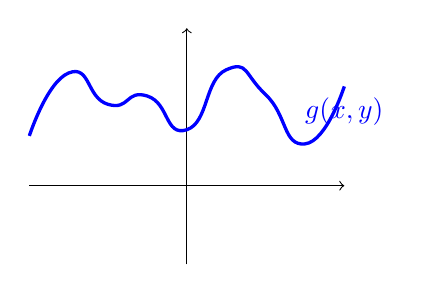
\begin{tikzpicture}
		\draw[->] (0,-1) -- (0,2);
		\draw[->] (-2,0) -- (2,0);

		\draw [blue, very thick]
		plot [smooth, tension=1, domain=-2:2, samples=9] (\x,{1+rand/2}) node[below] {$g(x,y)$};
	\end{tikzpicture}

	\paragraph{Διακριτού χρόνου / Διακριτό (discrete)}
	\begin{invitemize}
		\item \( t \) διακριτό \( \rightarrow \mathbb Z,\ n \in \mathbb Z \)
		\item \( g \) συνεχής \( \in \mathbb R  \)
	\end{invitemize}

	\begin{tikzpicture}[scale=0.7]
		\draw[->,gray] (0,0) -- (0,4.5);
		\draw[->,gray] (-6,0) -- (6,0);

		\foreach \x in {-5,...,5} {
			\draw (\x,0) node[below] {$\x$};
			\filldraw[black] (\x,0) -- (\x,{(1+rand)*2}) circle (1.5pt);
		};

		\draw (0,-1) node[below] {7\textsuperscript{ο} εξάμηνο};
	\end{tikzpicture}

	\paragraph{Κβαντισμένο}
	\begin{invitemize}
		\item \( n \in \mathbb Z \)
		\item \( g \) διακριτή
	\end{invitemize}
	\begin{tikzpicture}
	\draw[->,gray] (0,0) -- (0,4.5);
	\draw[->,gray] (-4,0) -- (4,0);

	\draw[gray,dashed] (-4,1) -- (4,1);
	\draw[gray,dashed] (-4,2) -- (4,2);
	\draw[gray,dashed] (-4,3) -- (4,3);

	\filldraw[black] (-3,0) node[below] {$-3$} -- (-3,1) circle (1.5pt);
	\filldraw[black] (-2,0) node[below] {$-2$} -- (-2,2) circle (1.5pt);
	\filldraw[black] (-1,0) node[below] {$-1$} -- (-1,1) circle (1.5pt);
	\filldraw[black] ( 0,0) node[below] {$0$} -- (0,0) circle (1.5pt);
	\filldraw[black] ( 1,0) node[below] {$1$} -- (1,1.5) circle (1.5pt);
	\filldraw[black] ( 2,0) node[below] {$2$} -- (2,3) circle (1.5pt);
	\filldraw[black] ( 3,0) node[below] {$3$} -- (3,2) circle (1.5pt);
	\draw (1,1) node[cross=10pt,red!50!black] {};
	\end{tikzpicture}

	\paragraph{Στοχαστικό}
	Περιέχει και τις τρεις κατηγορίες

	\subsection{Σύστημα}
	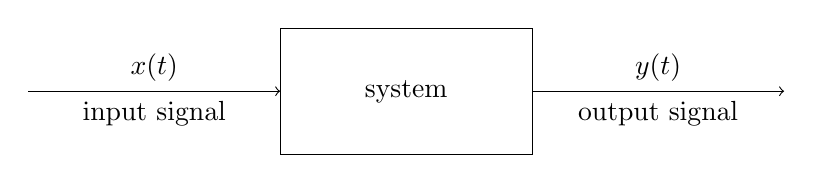
\begin{tikzpicture}[scale=0.8]
		\draw (-1,1) rectangle (3,-1) node[midway] {system};

		\draw[->] (-5,0) -- (-1,0) node[midway,above] {$x(t)$} node[midway,below] {input signal};
		\draw[->] (3,0) -- (7,0) node[midway,above] {$y(t)$} node[midway,below] {output signal};
	\end{tikzpicture}

	\subsection{Περιοδικά σήματα}
	Αν \( \exists T \in \mathbb R : \forall t \in \mathbb R \quad x(t)=x(t+T) \)
	τότε \( x(t) \) \textbf{περιοδικό σήμα} με περίοδο \( T \).

	Ή θα είναι 0, ή θα συνεχιστεί για πάντα.

	\[
	\int_{-\sfrac{T}{2}}^{\sfrac{T}{2}} x(t) \dif t =
	\int_{t_0-\sfrac{T}{2}}^{t_0+\sfrac{T}{2}} x(t) \dif t\ \forall t
	\]

	Η σύνθεση μιας συνάρτησης με μια περιοδική συνάρτηση είναι περιοδική;
	\subparagraph{Απόδ.}
		Έστω \(g\) μία περιοδική συνάρτηση:
		\begin{align*}
		\big(f\circ g\big)(x) &= f\left(g(x)\right) = f \left( g(x+T) \right) =
		\\ &= \big(f\circ g\big)(x+T)
		\end{align*}

	\subsection{Συμμετρίες}
	\begin{itemize}
	    \item Αν \( x(t) = x(-t) \ \forall t \) τότε η \( x(t) \) λέγεται \textbf{άρτια συνάρτηση} (even function).

	    \item Αν \( x(t) = -x(t) \ \forall t \) τότε η \( x(t) \) λέγεται \textbf{περιττή συνάρτηση} (odd function).
	\end{itemize}

	\paragraph{}
	Υποστηρίζω ότι κάθε συνάρτηση μπορεί να γραφεί σαν άθροισμα μιας άρτιας και μιας περιττής:

	\( \forall x(t) \quad \exists\ x_0(t), x_e(t): x(t) = x_e(t)+x_0(t) \)
	\subparagraph{Απόδ.}
	\begin{align*}
		x_e(t) &= \frac{x(t)+x(-t)}{2} \\
		x_o(t) &= \frac{x(t)-x(-t)}{2}.
	\end{align*}

	\paragraph{}
	\begin{align*}
		x{\underbrace{_e}_{\mathclap{\text{άρτια}}}}y_e &= z_e\\
		x_oy_o &=z_e \\
		x_ey_0 &=z_0 \\
		\int_{-A}^A x_0(t)\dif t &= 0 \\
		\int_{-\infty}^\infty x_0(t)\dif t &= ? \text{ (εξαρτάται)} \\
		\lim_{A\to \infty} \int_{-A}^A x_0(t)\dif t &= 0 \quad \text{(principal Cauchy value)}
	\end{align*}

	\subsection{Χαρακτηριστικά σήματα}
	\begin{enumpar}
		\item \textbf{Εκθετικό σήμα}
		\[
		x(t) = ce^{at}\quad a \in \mathbb R \quad c > 0
		\]
		\begin{tikzpicture}
		\draw[->,gray] (0,0) -- (0,4);
		\draw[->,gray] (-2,0) -- (4,0) node[below right] {$t$};

		\draw (1,3) node {$c > 0$};

		\draw[xscale=3,domain=-0.7:1.3,smooth,variable=\x,blue] plot ({\x},{exp(\x)});
		\draw[xscale=3,domain=1.3:-1.2,dashed,smooth,variable=\x,blue] plot ({\x},{exp(-\x)});
		\draw (4,1) node[anchor=north east,blue] {$a < 0$};
		\draw (4.5,3) node[anchor=north east,blue] {$a > 0$};
		\end{tikzpicture}
		\[
		x(t) = ce^{(\sigma t+j\omega)t} = ce^{\sigma t}e^{j\omega t}
		= ce^{\sigma t} \left[
		\cos(\omega t)+j\sin(\omega t)
		\right]
		\]

		\item \textbf{(Συν)ημιτονοειδή σήματα}
		\[
		x(t) = A \cos(\omega t\pm \phi)
		= a \mathrm{Re} \left\lbrace e^{j(\omega t +\phi)} \right\rbrace
		= A \frac{e^{j(\omega t \pm \phi)} + e^{-j(\omega t\pm \phi)}}{2}
		\]
		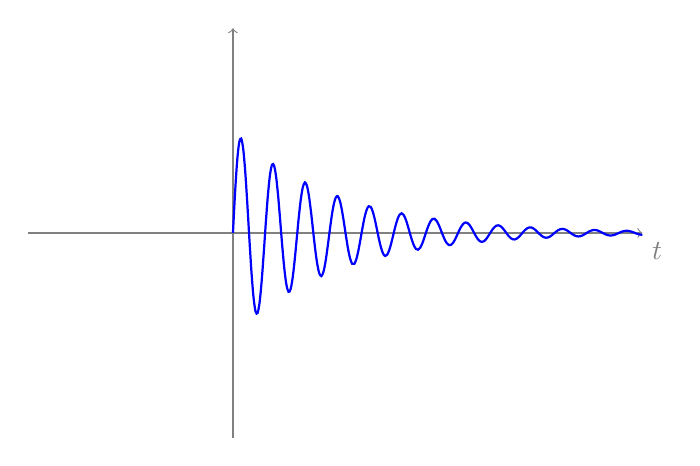
\begin{tikzpicture}[scale=1.3]
		\draw[->,gray] (0,-2) -- (0,2);
		\draw[->,gray] (-2,0) -- (4,0) node[below right] {$t$};


		\draw[scale=1,domain=0:4,samples=200,smooth,variable=\x,blue,thick] plot ({\x},{sin((\x r)*20)*exp(-\x)});
		\end{tikzpicture}

		\item \textbf{Δέλτα Dirac} \( \delta(t) \)

		\begin{tikzpicture}[scale=1.2]
		\draw[->,gray] (0,-2) -- (0,2) node[black,below right] {$\delta(t)$};
		\draw[->,gray] (-1,0) -- (1,0) node[below right] {$t$};
		\draw (0,0) node[below left] {$0$};

		\draw[very thick,blue,->] (0,0) -- (0,1);
		\end{tikzpicture}
		\begin{tikzpicture}[scale=1.2]
		\filldraw[fill=green!20] (-0.5,0) rectangle (0.5,1) node[above right] {$\sfrac{1}{T}$}
			node[midway,right] {$1$};

		\draw[->,gray] (0,-2) -- (0,2);
		\draw[->,gray] (-1.5,0) -- (2,0);

		\draw (current bounding box.east) node[above] {$\lim_{T\to0} P_T(t)=\delta(t)$};
		\end{tikzpicture}
		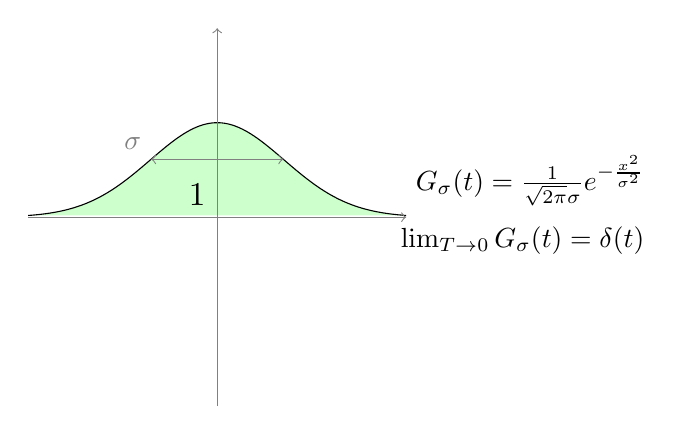
\begin{tikzpicture}[scale=1.2]
		\filldraw[scale=1,domain=-2:2,samples=200,smooth,variable=\x,fill=green!20]
			plot ({\x},{exp(-\x*\x)})
			node[above right] {$G_\sigma(t) = \frac{1}{\sqrt{2\pi}\sigma}e^{-\frac{x^2}{\sigma^2}} $}
			node[midway,above left] {$1$};

		\draw[->,gray] (0,-2) -- (0,2);
		\draw[->,gray] (-2,0) -- (2,0);

		\draw[<->,gray] (0.7,{exp(-pow(0.7,2))}) -- (-0.7,{exp(-pow(0.7,2))})
			node[above left] {$\sigma$};

		\draw (current bounding box.east) node[below left] {$\lim_{T\to0} G_\sigma(t)=\delta(t)$};
		\end{tikzpicture}
	    \paragraph{Ορ.}
	    \[
	    \int_{-\infty}^\infty f(t) \delta(t) \dif t = f(0)\ \forall f(t)
	    \]
	    \paragraph{}
	    \begin{align*}
	    \int_{-\infty}^\infty \delta(t)\dif t &=1 \\
	    \int_{-\infty}^\infty f(t)\delta(t-\tau) \dif t &= f(\tau) \\
	    \Aboxed{\int_{-\infty}^\infty f(\tau) \delta(t-\tau)\dif \tau &= f(t)} \\
	    \int_{-\infty}^\infty f(t)\delta(t-\tau)\dif \tau &= f(t)
	    \end{align*}

	    \begin{tikzpicture}[scale=2.5]
	    	\draw[->] (-0.5,0) -- (2,0) node[below] {$t$};
	    	\draw[->] (0,-0.2) -- (0,2);

	    	\draw [blue, very thick, mark position=0.7(c)]
	    	plot [smooth, tension=0.5, domain=-0.5:2, samples=9]
	    	(\x,{1+rand/2})
	    	node[below,right] {$f(t)$}
	    	;

	    	\draw[->,very thick] (c |- {(0,0)}) node[below] {$\tau$} -- (c);
	    	\filldraw (c) circle(.5pt);

	    	\draw[->] (-0.5,-3) -- (2,-3);
	    	\draw[->] (0,-3.2) -- (0,-1);

	    	\draw[->,very thick] let \p1=(c) in (c |- {(0,-3)}) node[below] {$\tau$}
	    	--  (\x1,-3cm+\y1) node[above] {$f(t)\delta(t-\tau)$};
	    	\filldraw (c) circle(.5pt);
	    \end{tikzpicture}

	    \paragraph[Ιδιότητες της δ(τ)]{Ιδιότητες της \( \delta(t) \)}
	    \begin{enumerate}
	    	\item \textbf{Κλιμάκωση}
	    	\[
	    	a \in \mathbb R: \delta(at) = \frac{1}{|a|}\delta(t)
	    	\]
	    	\subparagraph{Απόδ.}
	    	\[
	    	\underbrace{\int_{-\infty}^\infty \phi(t)\boxed{\delta(at)}\dif t}_{\mathclap{\begin{matrix}
	    			at=\xi\\\dif t = \frac{\dif \xi}{a}
	    			\end{matrix}}}
	    =
	    	\int_{-\infty_{(a)}}^{\infty_{(a)}} \phi\left( \frac{\xi}{a} \right) \delta(\xi)\frac{\dif \xi}{a}
	    	= \frac{1}{|a|}\int_{-\infty}^\infty \frac{\phi\left(\frac{\xi}{a} \right)}{|a|}\delta(\xi)\dif\xi = \frac{\phi(0)}{|a|}
	    	= \int_{-\infty}^\infty \phi(t)\boxed{\frac{\delta(t)}{|a|}}\dif t
	    	\]
	    	\item \(
	    	f(t)\delta(t)=f(0)\delta(t)
	    	\)
	    	\item \(
	    	f(t)\delta(t-\xi)=f(g)\delta(t-\xi)
	    	\)
    	\end{enumerate}
	\end{enumpar}

	\paragraph{}
	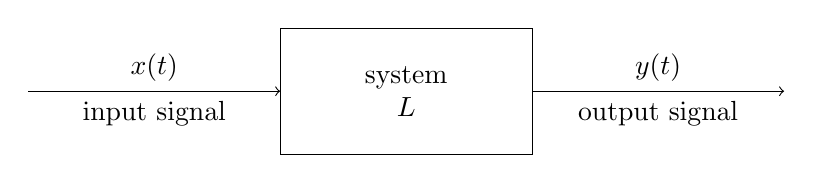
\begin{tikzpicture}[scale=0.8]
	\draw (-1,1) rectangle (3,-1) node[midway,style={align=center}] {system\\$\mathscr L$};

	\draw[->] (-5,0) -- (-1,0) node[midway,above] {$x(t)$} node[midway,below] {input signal};
	\draw[->] (3,0) -- (7,0) node[midway,above] {$y(t)$} node[midway,below] {output signal};
	\end{tikzpicture}

	Έστω \( \mathscr{L} \) το παραπάνω σύστημα (όχι ο μετασχηματισμός Laplace!), και:
	\begin{gather*}
		y(t) = \mathscr{L}\left\lbrace x(t) \right\rbrace \\
		\forall x_1(t)\ x_n(t)\\
		y_1(t) = \mathscr{L}\left\lbrace x_1(t) \right\rbrace \\
		y_2(t) = \mathscr{L}\left\lbrace x_2(t) \right\rbrace
	\end{gather*}

	Για const \( a_1, a_2 \in \mathbb R  \)
	\begin{align*}
	x(t) &= a_1x_1(t)+a_2x_2(t) \\
	y(t) &= \mathscr{L}\left\lbrace x(t) \right\rbrace \\
	\intertext{ανν}
	y(t) = a_1y_1(t)+a_2y_2(t) \\
	\intertext{τότε}
	\mathscr{L}: \text{ γραμμικό σύστημα}
	\end{align*}

	\begin{itemize}
		\item \(g(t) = \mathscr{L}\left\lbrace x(t) \right\rbrace\)

		\( x'(t)=x(t-\tau) \)

		ανν \( y'(t) = \mathscr{L} \left\lbrace x'(t) \right\rbrace
		= \mathscr{L} \left\lbrace x(t-\tau)^2 \right\rbrace = y(t-\tau)
		 \)

		 τότε το σύστημα \( \mathscr L \) είναι αμετάβλητο κατά τη μετατόπιση.

	\end{itemize}

	\paragraph{}

    \begin{tikzpicture}[scale=0.8]
    \draw (-1,-1) rectangle (3,1) node[above right] {$\mathscr L\left\lbrace\right\rbrace$} node[midway] {γραμμικό \& ΑΚΜ};

    \draw[->] (-5,0) -- (-1,0) node[midway,above] {$\delta(t)$} node[midway,below] {input signal};
    \draw[->] (3,0) -- (14,0) node[midway,above] {$\mathrm h(t)$}
	    node[midway,below] {κρουστική απόκριση (impulse response)};
    \end{tikzpicture}

    Υποστηρίζω ότι ένα γραμμικό \& ΑΚΜ σύστημα περιγράφεται πλήρως από την κρουστική
    απόκριση \( h(t) \).
    \subparagraph{Απόδ.} Από παραπάνω, γνωρίζουμε ότι
    \(
    x(t) = \int_{-\infty}^\infty x(t)\delta(t-\tau)\dif \tau
    \)
    \begin{align*}
    y(t) &= \mathscr L \left\lbrace x(t) \right\rbrace =
    \mathscr L \left\lbrace \int_{-\infty}^{\infty} x(t)\delta(t-\tau) \dif \tau
     \right\rbrace
     \\ & \overset{\text{linearity}}{=} \int_{-\infty}^{\infty} \mathscr L
     \left\lbrace x(t)\delta(t-\tau) \right\rbrace \dif\tau
     \\ &= \int_{-\infty}^{\infty} x(\tau) \mathscr L \left\lbrace
     \delta(t-\tau)
      \right\rbrace \dif \tau
      \\ & \underset{\underbrace{\text{TSI}}_{\text{Time shift invariant}}}{\overset{\text{ΑΚΜ}}{=}}
       \int_{-\infty}^{\infty} x(\tau) h(t-\tau)\dif \tau
       \\ y(t) &= \int_{-\infty}^{\infty}
        x(\tau)
        \underbrace{h(t-\tau)}_{\mathclap{\text{linear time-shift invariant}}}
        \dif\tau
    \end{align*}

    \paragraph{}

    \begin{itemize}
    	\item \( \delta(t)=\delta(-t) \) άρτια συνάρτηση
    	\item \( \delta^{(n)}(t) = \od[n]{}{t}\delta(t) \), για την οποία
    αποδεικνύεται ότι:
        \[
            \int_{-\infty}^{\infty} \delta^{(n)}(t)\phi(t)\dif t
            = (-1)^n\left.\phi^{(n)}(t)\right|_{t=0}
        \]
    \end{itemize}

    \subsection{Χρήσιμες Συναρτήσεις}

    \subsubsection{Βηματική Συνάρτηση (Unit Step Function)}
    \[
    \mathrm u(t) = \begin{cases}
    1 \quad & t > 0 \\
    0 \quad & t < 0
    \end{cases}
    \]
    \[
    \int_{-\infty}^{\infty} \mathrm u(t)\phi(t)\dif t =
    \mathscr N_{\mathrm u}\left\lbrace \phi(t) \right\rbrace =
    \underbrace{ \int_0^\infty \phi(t)\dif t}_{\mathclap{\text{number}}}
    \]
    \begin{tikzpicture}
    \begin{axis}[%
    xlabel=$t$
    ,ylabel=$\mathrm u(t)$
    ,axis lines = center
    ,ymax=1.5
    ,ytick={0,1}
    ,xtick={0,1}
    ]
    \addplot+[const plot, no marks,ultra thick] coordinates {(-4,0) (0,1) (4,1)};
    %\addplot+[const plot, no marks, thick] coordinates {(0,0) (1,0.25) (2,0.4) (3,0.5) (4,1) (4.49,1)} node[below=1.15cm,pos=.76,black] {$F_y$};
    \end{axis}
    \end{tikzpicture}

    \begin{align*}
    \delta(t) &= \od{}{t} \mathrm u(t)\\
    \mathrm u(t) &= \int_{-\infty}^t \delta(\tau)\dif\tau =
    \int_0^\infty \delta(t-\xi)\dif\xi
    \end{align*}

    \subsubsection{Ράμπα}
    \[
    \mathrm r(t) = \int_{-\infty}^t \mathrm u(\tau)\dif\tau =
    \begin{cases}
    t \quad & t \geq0 \\
    0 \quad & \text{else}
    \end{cases} = t\mathrm u(t)
    \]

    \begin{tikzpicture}
    	\draw[->] (0,-0.5) -- (0,4) node[right] {$\mathrm r(t)$};
    	\draw[->] (-2,0) -- (4,0) node[below] {$t$};

    	\draw (0,0) node[below right] {$0$};

    	\draw[very thick,blue] (-2,0) -- (0,0) -- (3.5,3.5);
    \end{tikzpicture}

    \[
    \mathrm u(t) =\od{}{t} \mathrm r(t)
    \]

    \subsubsection{Ορθογωνικός παλμός (Rectangular Pulse function)}
    \[
    \mathrm p_a(t) = \begin{cases}
    1 &\quad |t| < a \\
    0 &\quad |t| > a
    \end{cases}
    \]

    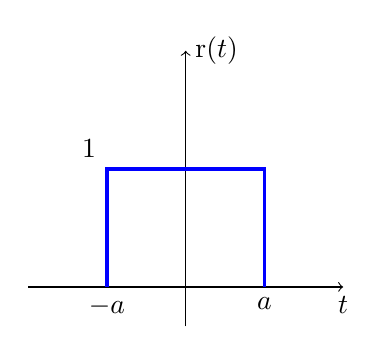
\begin{tikzpicture}
    \draw[->] (0,-0.5) -- (0,3) node[right] {$\mathrm r(t)$};
    \draw[->] (-2,0) -- (2,0) node[below] {$t$};

    \draw[very thick,blue]
	    (-1,0) node[below,black] {$-a$} --
	    (-1,1.5) node[above left, black] {$1$} --
	    (1,1.5) --
	    (1,0) node[below,black] {$a$};
    \end{tikzpicture}

    \subparagraph{}

    \begin{tikzpicture}
    \draw[->] (0,-0.5) -- (0,2);
    \draw[->] (-2,0) -- (3,0) node[below] {$t$};

    \draw[very thick,blue]
    (-3,0) --
    (-1,0) node[below,black] {$-a$} --
    (-1,1) --
    (3,1) node[above right] {$\mathrm u(t+a)$};
    \end{tikzpicture}
    \begin{tikzpicture}
    \draw[->] (0,-0.5) -- (0,2);
    \draw[->] (-2,0) -- (3,0) node[below] {$t$};

    \draw[very thick,blue]
    (-3,0) --
    (1,0) node[below,black] {$a$} --
    (1,1) --
    (3,1) node[above right] {$\mathrm u(t-a)$};
    \end{tikzpicture}

    \begin{align*}
    \mathrm p_a(t) =& \mathrm u(t+a) - \mathrm u(t-a) \\
    \od{}{t} \mathrm p_a(t) =& \delta(t+a)-\delta(t-a)
    \end{align*}

    \begin{tikzpicture}
    \draw[->] (0,-0.5) -- (0,3) node[right] {$\od{}{t}\mathrm p_a(t)$};
    \draw[->] (-2,0) -- (2,0) node[below] {$t$};

    \draw[very thick,blue,->]
    (-1,0) node[below,black] {$-a$} --
    (-1,1.5) node[above] {$\delta(t+a)$};

    \draw[very thick,blue,->]
    (1,0) node[above,black] {$a$} --
    (1,-1.5) node[below] {$-\delta(t-a)$};
    \end{tikzpicture}

    \subsubsection{Τριγωνικός Παλμός (Triangular Pulse function)}
    \[
    \mathrm p_{\mathrm{tr},a} = \begin{cases}
    1-\frac{|t|}{a} &\quad |t|<a \\
    0 &\quad |t|>a
    \end{cases}
    \]
    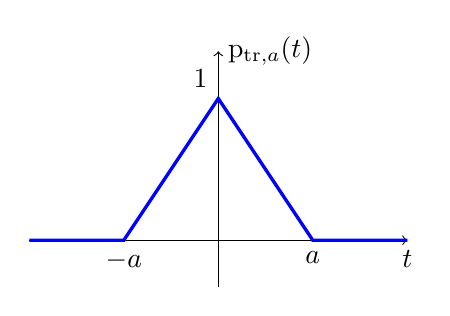
\begin{tikzpicture}[scale=1.2]
    \draw[->] (0,-0.5) -- (0,2) node[right] {$\mathrm p_{\mathrm{tr},a}(t)$};
    \draw[->] (-2,0) -- (2,0) node[below] {$t$};

    \draw[very thick,blue]
    (-2,0) --
    (-1,0) node[below,black] {$-a$} --
    (0,1.5) node[above left, black] {$1$} --
    (1,0) node[below,black] {$a$} --
    (2,0);
    \end{tikzpicture}
    \[
    p_{\mathrm{tr},a}(t) = \frac{1}{a} \left[
        \mathrm r(t+a) + \mathrm r(t-a) - 2\mathrm r(t)
    \right]
    \]
    \begin{tikzpicture}[scale=0.7]
    	\draw[gray] (-4,0) -- (4,0);
    	\draw[gray] (0,-4) -- (0,4);

    	\draw[dashed] (-2,0) -- (1,3);
    	\draw[dashed] (2,0) -- (4,2);
    	\draw[dashed] (0,0) -- (2,-4);

    	\draw[blue,opacity=.3,very thick] (-4,0) -- (-2,0) -- (0,2) -- (2,0) -- (4,0);
    \end{tikzpicture}

    \subsection{Χαρακτηριστικά Μεγέθη}
    \begin{enumpar}
    	\item \textbf{Μέση τιμή (Mean Value)}
    	\[
    	\overline{x(t)} = \frac{1}{t_2-t_1} \int_{t_1}^{t_2}x(t)\dif t
    	\]

    	Αν περιοδική τότε \begin{align*}
    	\bar x(t) &= \frac{1}{T} \int_0^T x(t)\dif t \\
    	&= \frac{1}{T} \int_{t_0}^{t_0+T} x(t)\dif t
    	\end{align*}
    	\item \textbf{Ενεργός τιμή (Root Mean Square Value)}
    	\[
    	\overline{\overline{x(t)}} = \left[
    	    \frac{1}{t_2-t_1}\int_{t_1}^{t_2} x^2(t)\dif t
    	\right]^{\sfrac{1}{2}}
    	\]
    	Αν ημιτονοειδές σήμα \(\bar{\bar{x}}(t) = \frac{x_{\max}}{\sqrt{2}}
    	\)

    	\item \textbf{Ενέργεια - Ισχύς}
    	\begin{itemize}
    		\item Στιγμιαία ισχύς (Instant power)
    		\[
    		p(t) = x^2(t)
    		\]
    		\item Μέση ισχύς (Mean power)
    		\[
    		\overline{p(t)} = \frac{1}{t_2-t_1}\int_{t_1}^{t_2}x^2(t)\dif t
    		= \left( \overline{\overline{x(t)}} \right)^2
    		\]
    		\item Ενέργεια (Energy)
    		\[
    		W = \int_{t_1}^{t_2} p(t) \dif t =
    		\int_{t_1}^{t_2} x^2(t)\dif t = (t_2-t_1)\left(
    		\overline{\overline{x(t)}}
    		\right)^2
    		\]
    	\end{itemize}

    	\textbf{Σήματα} \( \begin{dcases}
    	\text{\textbf{Σήμα ενέργειας} αν} \lim_{T\to \infty}W< \infty
    	\\ \\
    	\text{\textbf{Σήμα ισχύος} αν} \lim_{T\to \infty}\overline{p(t)}>0
	    \\ \text{Υπάρχουν και σήματα που δεν είναι ούτε ενέργειας, ούτε ισχύος.}
    	\end{dcases}
    	\)
    \end{enumpar}

    \subsection{Συνέλιξη}
    \[ x(t) = \int_{-\infty}^{\infty}x(t)\delta(t-\tau)d\tau \]
    \begin{tikzpicture}[scale=0.7]
    \draw (-1,-1) rectangle (3,1) node[above right] {$\mathscr L\left\lbrace\right\rbrace$} node[midway,align=center]
    {γραμμικό\\ \& \\ ΑΚΜ};

    \draw[->] (-5,0) -- (-1,0) node[midway,above] {$\delta(t)$} node[midway,below] {input signal};
    \draw[->] (3,0) -- (9,0) node[midway,above] {$\mathrm h(t)$}
    node[midway,below,align=center] {κρουστική απόκριση\\ (impulse response)};
    \end{tikzpicture}
    \[ h(t)=\mathscr L\left\lbrace \delta(t) \right\rbrace \]
    \[ y(t) = \int_{-\infty}^{\infty} x(\tau)h(t-\tau)\dif\tau
    = \underbrace{x(t)}_{\mathclap{\text{είσοδος}}}
    \overset{\substack{\text{συνέλιξη}\\\uparrow}}{*}
    \underbrace{h(t) }_{\mathclap{\text{κρουστική απόκριση}}}\]

    \paragraph{Συνέλιξη - Convolution}
    \[
    z(t)=x(t)*y(t)=\int_{-\infty}^{\infty} x(\tau)y(t-\tau)\dif\tau
    \]

    \paragraph{}
    \begin{itemize}
    	\item \(x(t)*y(t)=y(t)*x(t)\) \textbf{Αντιμεταθετική}
    	\subparagraph{}
    	\[
    	\int_{-\infty}^{\infty} x(\tau)y(t-\tau)\dif\tau
    	= \int_{-\infty}^{\infty} x(t-\lambda)y(\lambda)[-\dif\lambda]
    	= \int_{-\infty}^{\infty} y(\lambda)x(t-\lambda)\dif\lambda
    	= y(t)*x(t)
    	\]
    	\item \( x_1(t)*\left[x_2(t)*x_3(t)\right] =
    	\left[x_1(t)*x_2(t)\right]*x_3(t) \) \textbf{Προσεταιριστική}
    \end{itemize}

    \paragraph{Παρ.}
    \begin{align*}
    f_1(t) &= 2(1-t)\left[ \mathrm u(t)-u(t-1) \right] \\
    f_2(t) &= \mathrm u(t) - \mathrm u(t-2)
    \end{align*}

    \subparagraph{Γραφική μέθοδος υπολογισμού συνέλιξης}
    \hspace{0pt}
    \\

    \begin{tikzpicture}[every node/.style={black}]
	    \draw (0,3) -- (0,-3.5);

    	\draw (-3,0) -- (3,0) node[below] {$\tau$};
    	\draw (-3,-3) -- (3,-3) node[below] {$\tau$};

    	\draw[very thick,blue] (0,2)
    	node[left] {$2$}
    	node[above right,black] {$f_1(\tau)$}
    	-- (1,0) node[below] {$1$};

    	\draw[very thick,blue] (0,-2)
    	node[left] {$1$}
    	node[above right,black] {$f_2(\tau)$}
    	-- (2,-2) -- (2,-3) node[below] {$2$};
    	\draw[dashed] (1,-3) node[below] {$1$} -- (1,-2);
    \end{tikzpicture}


    \begin{tikzpicture}[every node/.style={black}]
    	\draw (-3,0) -- (3,0) node[below] {$\tau$};
    	\draw[->] (0,-1) -- (0,2);

    	\draw[very thick,blue]
    	(-2,0) node[below] {$-2$}
    	-- (-2,1)
    	-- (0,1) node[above right,blue] {$f_2(-\tau)$}
    	-- (0,0) node[below left] {$0$}
    	;
    \end{tikzpicture}


    \begin{tikzpicture}[every node/.style={black}]
    \draw (-3,0) -- (3,0) node[below] {$\tau$};
    \draw[->] (0,-1) -- (0,2);

    \draw[very thick,blue]
    (-0.8,0)
    -- (-0.8,1)
    -- (1.2,1) node[above right,blue] {$f_2(t-\tau)$}
    -- (1.2,0)
    ;

    \draw[<->] (0,1.4) -- (1.2,1.4) node[midway,fill=white,inner sep=2pt] {$t$};
    \end{tikzpicture}

    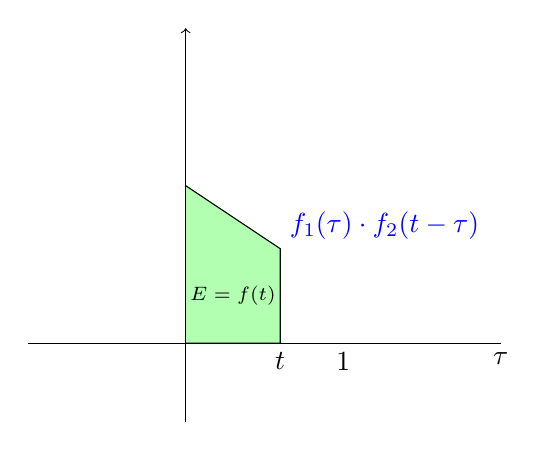
\begin{tikzpicture}[every node/.style={black},scale=2]
    \filldraw[fill=green!30]
    (0,1)
    -- (0.6,0.6)  node[above right,blue] {$f_1(\tau)\cdot f_2(t-\tau)$}
    -- (0.6,0) node[below] {$t$}
    -- (0,0);

    \draw (0.3,0.3) node {\scriptsize $E=f(t)$};
    \draw(1,0) node[below] {$1$};

    \draw (-1,0) -- (2,0) node[below] {$\tau$};
    \draw[->] (0,-0.5) -- (0,2);
    \end{tikzpicture}

    \begin{itemize}
    	\item \(t<0\)
    	\begin{tikzpicture}[baseline={([yshift=-.8ex]current bounding box.center)}]
    		\draw (-2,0) -- (2,0);
    		\draw (0,-0.2) -- (0,1.5);
    		\draw[very thick,blue] (0,1) -- (1,0);

    		\draw (-2,-2) -- (2,-2);
    		\draw (0,-2.2) -- (0,-0.5);
    		\draw[very thick,blue] (-1.8,-2) -- (-1.8,-1.2) -- (-0.3,-1.2) -- (-0.3,-2);
    	\end{tikzpicture}
    	\(f(t) = 0\)

    	\item \(0<t<1\)
    	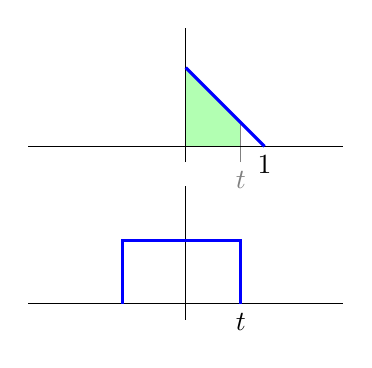
\begin{tikzpicture}[baseline={([yshift=-.8ex]current bounding box.center)}]
    	\fill[green!30] (0,1) -- (0.7,0.3) -- (0.7,0) -- (0,0);
    	\draw[gray] (0.7,-0.2) node[below] {$t$} -- (0.7,0) -- (0.7,0.3);

    	\draw (-2,0) -- (2,0);
    	\draw (0,-0.2) -- (0,1.5);
    	\draw[very thick,blue] (0,1) -- (1,0);
    	\draw (1,0) node[below] {$1$};

    	\draw (-2,-2) -- (2,-2);
    	\draw (0,-2.2) -- (0,-0.5);
    	\draw[very thick,blue] (-0.8,-2) -- (-0.8,-1.2) -- (0.7,-1.2) -- (0.7,-2);
    	\draw(0.7,-2) node[below]{$t$};
    	\end{tikzpicture}
    	\(f(t) =  \frac{1}{2}(2+2-2t)t=(2-t)t \)

    	\item \(1<t<2\)
    	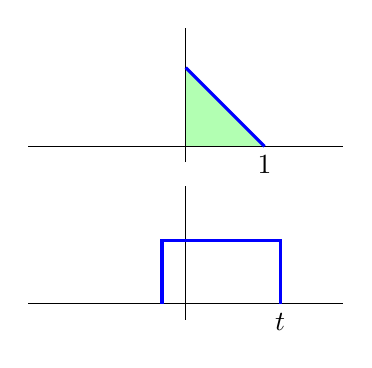
\begin{tikzpicture}[baseline={([yshift=-.8ex]current bounding box.center)}]
    	\fill[green!30] (0,1) -- (1,0) -- (0,0);

    	\draw (-2,0) -- (2,0);
    	\draw (0,-0.2) -- (0,1.5);
    	\draw[very thick,blue] (0,1) -- (1,0);
    	\draw (1,0) node[below] {$1$};

    	\draw (-2,-2) -- (2,-2);
    	\draw (0,-2.2) -- (0,-0.5);
    	\draw[very thick,blue] (-0.3,-2) -- (-0.3,-1.2) -- (1.2,-1.2) -- (1.2,-2);
    	\draw(1.2,-2) node[below]{$t$};
    	\end{tikzpicture}
    	\(f(t) =  1 \)

    	\item \(2<t<3\)
    	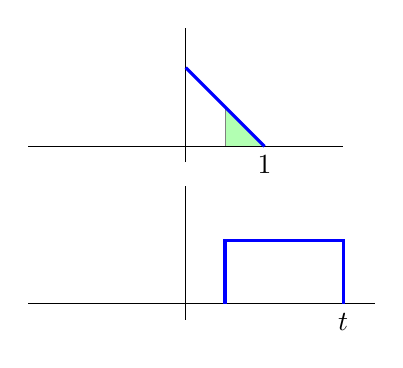
\begin{tikzpicture}[baseline={([yshift=-.8ex]current bounding box.center)}]
    	\fill[green!30] (0.5,0.5) -- (1,0) -- (0.5,0);
    	\draw[gray] (0.5,0) -- (0.5,0.5);

    	\draw (-2,0) -- (2,0);
    	\draw (0,-0.2) -- (0,1.5);
    	\draw[very thick,blue] (0,1) -- (1,0);
    	\draw (1,0) node[below] {$1$};

    	\draw (-2,-2) -- (2.4,-2);
    	\draw (0,-2.2) -- (0,-0.5);
    	\draw[very thick,blue] (0.5,-2) -- (0.5,-1.2) -- (2,-1.2) -- (2,-2);
    	\draw(2,-2) node[below]{$t$};
    	\end{tikzpicture}
    	\(f(t) = \frac{(t-1)\cdot2\cdot\left(1-(t-2)\right)}{2}=(t-1)(3-t) \)

    	\item \(t>3\)
    	\begin{tikzpicture}[baseline={([yshift=-.8ex]current bounding box.center)}]
    	\draw (-2,0) -- (2,0);
    	\draw (0,-0.2) -- (0,1.5);
    	\draw[very thick,blue] (0,1) -- (1,0);
    	\draw (1,0) node[below] {$1$};

    	\draw (-2,-2) -- (3.4,-2);
    	\draw (0,-2.2) -- (0,-0.5);
    	\draw[very thick,blue] (1.2,-2) -- (1.2,-1.2) -- (2.7,-1.2) -- (2.7,-2);
    	\end{tikzpicture}
    	\(f(t) = 0 \)
    \end{itemize}
    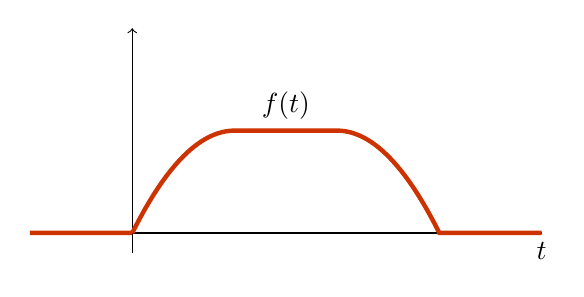
\begin{tikzpicture}[scale=1.3]
    	\draw[->] (0,-0.2) -- (0,2);
    	\draw (-1,0) -- (4,0) node[below] {$t$};

    	\draw[ultra thick,red!80!green]
    	(-1,0)
    	-- (0,0)
    	plot[domain=0:1] (\x,{(2-\x)*\x})
    	-- (2,1) node[above,midway,black] {$f(t)$}
    	plot[domain=2:3] (\x,{(\x-1)*(3-\x)})
    	-- (4,0)
    	;
    \end{tikzpicture}

    \subparagraph{Αναλυτική μέθοδος}
    \hspace{0pt}

    Παρατηρώ ότι: \[
    \int_{-\infty}^{\infty} f(t,\tau) \mathrm u(\tau-\xi)\mathrm u(\phi-\tau)\dif\tau
    = \int_{\xi}^\phi f(t,\tau)\dif\tau\mathrm u(\phi-\xi)
    \]

	{
	\setlength{\mathindent}{-10cm}
    \begin{align*}
    f(t) &= \int_{-\infty}^{\infty}
    \underbrace{2(1-\tau)}_{\mathclap{x(\tau)}}\left[\mathrm u(\tau)-\mathrm u(\tau+1) \right]\left[
    \mathrm u(t-\tau)-\mathrm u(t-\tau-2)
    \right] \dif\tau \\
    &= \int_{-\infty}^{\infty} x(\tau) \left[
    \mathrm u(\tau)\mathrm u(t-\tau)-\mathrm u(\tau-1)\mathrm u(t-\tau)
    -\mathrm u(\tau)\mathrm u(t-\tau-2)+\mathrm u(\tau-1)\mathrm u(t-\tau-2)
    \right]\dif\tau \\
    &= \int_0^t x(\tau)\dif\tau\mathrm u(t)
    -\int_1^x x(\tau)\dif\tau \mathrm u(t-1)
    -\int_0^{t-2}x(\tau)\dif\tau \mathrm u(t-2)
    +\int_1^{t-2}x(\tau)\dif\tau\mathrm u(t-3)
    \\ &=
    (2t-t^2)\mathrm u(t) - \left[2t-t^2-1\right]\mathrm u(t-1)
    - \left[ 2(t-2)-(t-2)^2 \right] \mathrm u(t-2)+
    \left[
    2(t-2)-(t-2)^2-1
    \right] \mathrm u(t-3)
    \end{align*}
	}

    \paragraph{Ex}
    \begin{align*}
    f_1(t) &= e^t\mathrm u(-t) \\
    f_2(t) &= \mathrm u(-t+2) \\
    f &= f_1*f_2
    \end{align*}
    \begin{align*}
    f &= \int_{-\infty}^{\infty}  e^\tau \mathrm u(-\tau)
    \mathrm u\left( -(t-\tau)+2 \right)\dif\tau
    \\&= \int_{-\infty}^{\infty} e^\tau \mathrm u(-\tau)
    \mathrm u(\tau-t+2)\dif\tau
    \\ &= \int_{-\infty}^{\infty} e^\tau \mathrm u(\tau)\mathrm u(-t+2-\tau)\dif\tau
    \\&= \int_{t-2}^0 e^\tau\dif\tau\mathrm u(2-t)
    \\&= \left. e^\tau \right|_{t-2}^0\mathrm u(2-t)
    \\&=\left[ 1-e^{t-2} \right]\mathrm u(2-t)
    \end{align*}

	\paragraph{}
	\begin{align*}
	\int_{-\infty}^{\infty} f(t,\tau)\mathrm u(\tau-\xi)\mathrm u(\phi-\tau)\dif\tau
	=\int_\xi^\phi f(t,\tau)\dif \tau \mathrm u(\phi-\xi)
	\end{align*}

	\paragraph{Ex.} \hspace{0pt}\\


	\begin{tikzpicture}
		\draw (-3,0) -- (3,0);
		\draw (0,-2) -- (0,2);

		\draw[very thick,blue,->] (0,0) node[below left,black] {$0$}
		-- (0,1) -- (-1,1) node[above,midway] {$\mathrm u(-\tau)$};

		\draw[very thick,blue,->] (-1.4,0) node[below,black] {$t+2$}
		-- (-1.4,0.6) -- (-2.6,0.6);

		\draw[very thick,blue,->] (1.4,0) node[below,black] {$t+2$}
		-- (1.4,0.6) -- (0.2,0.6);
	\end{tikzpicture}

	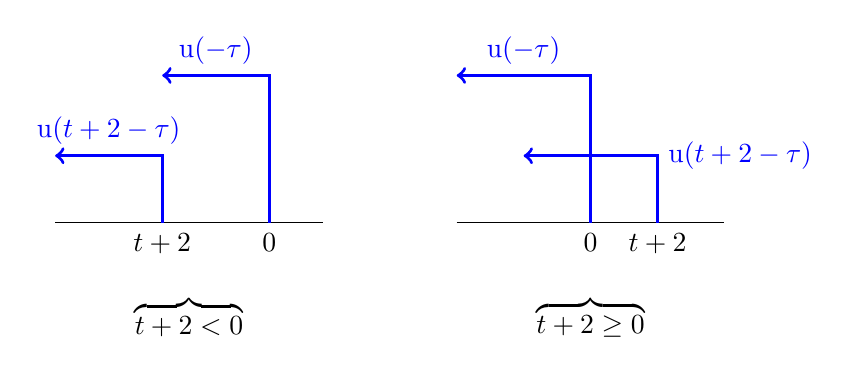
\begin{tikzpicture}[scale=1.7]
		\draw (-4,0) -- (-2,0);
		\draw[very thick,blue,->] (-3.2,0) node[below,black] {$t+2$}
		-- (-3.2,0.5) -- (-4,0.5) node[above,midway] {$\mathrm u(t+2-\tau)$};
		\draw[very thick,blue,->] (-2.4,0) node[below,black] {$0$}
		-- (-2.4,1.1) -- (-3.2,1.1) node[above,midway] {$\mathrm u(-\tau)$};
		\draw (-3,-0.7) node {$\overbrace{t+2<0}$};

		\draw (-1,0) -- (1,0);
		\draw[very thick,blue,->] (0.5,0) node[below,black] {$t+2$}
		-- (0.5,0.5) node[right] {$\mathrm u(t+2-\tau)$} -- (-0.5,0.5);
		\draw[very thick,blue,->] (0,0) node[below,black] {$0$}
		-- (0,1.1) -- (-1,1.1) node[above,midway] {$\mathrm u(-\tau)$};
		\draw (0,-0.7) node {$\overbrace{t+2\geq0}$};
	\end{tikzpicture}

	\begin{align*}
	x(t) &= e^t\mathrm u(-t) \\
	y(t) &= \mathrm u(t+2) \\
	z(t) &= x(t)*y(t) = \int_{-\infty}^{\infty} e^\tau \mathrm u(-\tau)
	\mathrm u \left[(t-\tau)+2\right]\dif\tau
	= \int_{-\infty}^{\infty} e^\tau \mathrm u(-\tau)\mathrm u(t+2-\tau)\dif\tau
	\\ &= \int_{-\infty}^{\infty} e^\tau\left[1-\mathrm u(t)\right]
	\mathrm u(t+2-\tau)\dif \tau \\ &=
	\int_{-\infty}^{\infty} e^\tau \mathrm u(t+2-\tau)\dif\tau-
	\int_{-\infty}^{\infty} e^\tau \mathrm u(\tau)u(t+2-\tau)\dif\tau
	\\ &= \int_{-\infty}^{t+2}e^\tau\dif \tau
	\cancelto{1}{\mathrm u\left(t+2-(-\infty)\right)} - \int_0^{t+2}
	e^\tau\dif\tau \mathrm u(t+2)
	\\ &= e^{t+2}-\left[ e^{t+2}- 1 \right]\mathrm u(t+2)
	\end{align*}

	\paragraph{Ex.}
	\begin{align*}
	x(t) &= e^t\mathrm u(-t) \\
	y(t) &= \mathrm u(t+2)-\mathrm u(t+1) \\
	z(t) &= x(t) * y(t) = \int_{-\infty}^{\infty} x(\tau)y(t-\tau)\dif\tau
	= \int_{-\infty}^{\infty} e^\tau\mathrm u(-\tau)\left[
	\mathrm u(t-\tau+2)-\mathrm u(t-\tau+1)
	\right]\dif\tau
	\\ &= \int_{-\infty}^{\infty} e^\tau
	\mathrm u(-\tau)\mathrm u(t-\tau+2)\dif\tau - \int_{-\infty}^{\infty}
	e^\tau \mathrm u(-\tau)\mathrm u(t-\tau+1)\dif\tau
	\\ &= \int_{-\infty}^{\infty} e^\tau
	\left[ 1-\mathrm u(\tau) \right]\mathrm u(t-\tau+2)\dif\tau -
	\int_{-\infty}^{\infty} e^\tau \left[ 1-\mathrm u(\tau) \right]
	\mathrm u(t-\tau+1)\dif\tau
	\\ &= \int_{-\infty}^{\infty}
	\mathsmaller{e^\tau \mathrm u(t-\tau+2)\dif\tau}
	- \int_{-\infty}^{\infty}
	\mathsmaller{\mathsmaller{
		 e^\tau \mathrm u(\tau) \mathrm u(t-\tau+2)\dif\tau}}
	- \int_{-\infty}^{\infty}
	\mathsmaller{\mathsmaller{ e^\tau \mathrm u(t-\tau+1)\dif\tau}}
	+ \int_{-\infty}^{\infty}\mathsmaller{\mathsmaller{
		 e^\tau \mathrm u(\tau)\mathrm u(t-\tau+1)\dif\tau}}
	\\ &= \int_{-\infty}^{t+1} e^\tau\dif\tau - \int_{-\infty}^{t+1}e^\tau\dif\tau
	- \int_0^{t+2}e^\tau\dif\tau\mathrm u(t+2)
	+ \int_0^{t+1}e^\tau\dif\tau \mathrm u(t+1)
	\\ &= \int_{t+1}^{t+2}e^\tau\dif\tau
	-\left[ e^{t+2}-1 \right]\mathrm u(t+2)
	+\left[ e^{t+1}-1 \right]\mathrm u(t+1)
	\end{align*}

	\vspace{1cm}
	\paragraph{}
	\( \exists h(t) \) ανν LTI
	\begin{align*}
		y(t) &= x(t)*h(t) \\ &=\int_{-\infty}^{\infty} x(\tau)h(t-\tau)\dif\tau
		\\ &= \int_{-\infty}^{\infty} h(\tau)x(t-\tau)\dif\tau
	\end{align*}

	Έστω ότι η \( x(t) = e^{j\omega t} \)
	\begin{align*}
	y(t) &= \int_{-\infty}^{\infty} h(t) e^{j\omega(t-\tau)}\dif\tau
	= e^{j\omega t} \int_{-\infty}^{\infty} h(\tau)e^{-j\omega\tau}\dif\tau
	\\ &= x(t)\underbrace{\int_{-\infty}^{\infty} h(\tau)e^{-j\omega\tau}\dif\tau}_{\mathclap{h(t) \xrightarrow{FT} H(\omega)}}
	\end{align*}

	\begin{align*}
	x(t) &= A_1e^{j\omega_1 t} + A_2e^{j\omega_2 t} \\
	y(t) &= A_1e^{j\omega_1 t}H(\omega_1)+A_2e^{j\omega_2t}H(\omega_2)
	\end{align*}
